% gerado por scripts/build_paper_assets.py -- nao editar a mao
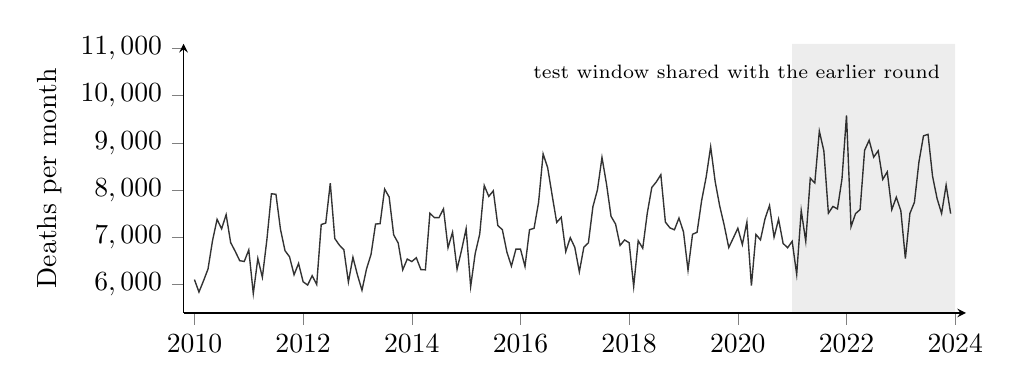
\begin{tikzpicture}
\begin{axis}[
  width=0.95\textwidth, height=5.0cm,
  xlabel={}, ylabel={Deaths per month},
  xmin=2009.8, xmax=2024.2, ymin=5400, ymax=11100,
  xtick={2010,2012,2014,2016,2018,2020,2022,2024},
  xticklabel style={/pgf/number format/1000 sep=},
  % sem isto o pgfplots troca o eixo por \cdot 10^4, que e ilegivel aqui
  scaled y ticks=false,
  ytick={6000,7000,8000,9000,10000,11000},
  yticklabel style={/pgf/number format/fixed, /pgf/number format/1000 sep={,}},
  axis lines=left, tick align=outside, tick pos=left,
  every axis plot/.append style={line width=0.5pt},
]
\addplot[draw=black!80, mark=none] coordinates {(2010.0000,6107) (2010.0833,5843) (2010.1667,6079) (2010.2500,6332) (2010.3333,6934) (2010.4167,7382) (2010.5000,7182) (2010.5833,7481) (2010.6667,6890) (2010.7500,6706) (2010.8333,6507) (2010.9167,6490) (2011.0000,6735) (2011.0833,5811) (2011.1667,6554) (2011.2500,6156) (2011.3333,6952) (2011.4167,7924) (2011.5000,7913) (2011.5833,7172) (2011.6667,6719) (2011.7500,6590) (2011.8333,6208) (2011.9167,6448) (2012.0000,6060) (2012.0833,5991) (2012.1667,6189) (2012.2500,6004) (2012.3333,7272) (2012.4167,7304) (2012.5000,8148) (2012.5833,6976) (2012.6667,6837) (2012.7500,6738) (2012.8333,6054) (2012.9167,6579) (2013.0000,6205) (2013.0833,5881) (2013.1667,6331) (2013.2500,6640) (2013.3333,7283) (2013.4167,7291) (2013.5000,8023) (2013.5833,7855) (2013.6667,7054) (2013.7500,6880) (2013.8333,6314) (2013.9167,6542) (2014.0000,6488) (2014.0833,6569) (2014.1667,6318) (2014.2500,6313) (2014.3333,7512) (2014.4167,7418) (2014.5000,7417) (2014.5833,7605) (2014.6667,6781) (2014.7500,7110) (2014.8333,6327) (2014.9167,6734) (2015.0000,7184) (2015.0833,5958) (2015.1667,6658) (2015.2500,7069) (2015.3333,8099) (2015.4167,7868) (2015.5000,7986) (2015.5833,7251) (2015.6667,7163) (2015.7500,6690) (2015.8333,6392) (2015.9167,6753) (2016.0000,6753) (2016.0833,6385) (2016.1667,7164) (2016.2500,7192) (2016.3333,7743) (2016.4167,8767) (2016.5000,8479) (2016.5833,7890) (2016.6667,7317) (2016.7500,7426) (2016.8333,6700) (2016.9167,6994) (2017.0000,6788) (2017.0833,6271) (2017.1667,6794) (2017.2500,6884) (2017.3333,7651) (2017.4167,8009) (2017.5000,8694) (2017.5833,8130) (2017.6667,7446) (2017.7500,7282) (2017.8333,6830) (2017.9167,6946) (2018.0000,6886) (2018.0833,5960) (2018.1667,6930) (2018.2500,6769) (2018.3333,7511) (2018.4167,8057) (2018.5000,8175) (2018.5833,8328) (2018.6667,7325) (2018.7500,7202) (2018.8333,7161) (2018.9167,7409) (2019.0000,7117) (2019.0833,6307) (2019.1667,7067) (2019.2500,7108) (2019.3333,7776) (2019.4167,8274) (2019.5000,8919) (2019.5833,8180) (2019.6667,7664) (2019.7500,7254) (2019.8333,6785) (2019.9167,6987) (2020.0000,7194) (2020.0833,6848) (2020.1667,7324) (2020.2500,5978) (2020.3333,7062) (2020.4167,6948) (2020.5000,7392) (2020.5833,7678) (2020.6667,7005) (2020.7500,7385) (2020.8333,6872) (2020.9167,6781) (2021.0000,6917) (2021.0833,6217) (2021.1667,7569) (2021.2500,6917) (2021.3333,8253) (2021.4167,8153) (2021.5000,9251) (2021.5833,8830) (2021.6667,7512) (2021.7500,7656) (2021.8333,7603) (2021.9167,8237) (2022.0000,9582) (2022.0833,7227) (2022.1667,7504) (2022.2500,7589) (2022.3333,8846) (2022.4167,9057) (2022.5000,8699) (2022.5833,8834) (2022.6667,8228) (2022.7500,8388) (2022.8333,7588) (2022.9167,7850) (2023.0000,7563) (2023.0833,6551) (2023.1667,7507) (2023.2500,7745) (2023.3333,8600) (2023.4167,9151) (2023.5000,9183) (2023.5833,8297) (2023.6667,7823) (2023.7500,7507) (2023.8333,8107) (2023.9167,7504)};
\addplot[draw=none, fill=black, fill opacity=0.07, forget plot]
  coordinates {(2021.0,5400) (2024.0,5400) (2024.0,11100) (2021.0,11100)} \closedcycle;
% ancorado a direita e dentro do limite do eixo: centralizado em 2022.5 o rotulo
% estourava a borda e saia cortado
\node[anchor=east, font=\scriptsize, text=black]
  at (axis cs:2023.9,10500) {test window shared with the earlier round};
\end{axis}
\end{tikzpicture}